{\ttfamily oomph-\/lib} does not provide its own unstructured mesh generator but has several mesh classes that generate unstructured meshes from the output of third-\/party unstructured mesh generators.

{\bfseries Notes\+:}
\begin{DoxyEnumerate}
\item The unstructured tet and triangle meshes listed below can {\bfseries not} be used with {\ttfamily oomph-\/lib\textquotesingle{}s} mesh adaptation or node-\/update procedures. A suitably fine mesh has to be generated offline by the third-\/party mesh generator. If required, node-\/updates (in response to changes in the domain boundaries) have to be performed manually. ~\newline
~\newline

\item For some element types, the mesh generation process is not particularly efficient (yet!). A suitable warning message is issued in such cases. ~\newline
~\newline

\item Since the third-\/party mesh generators tend to triangulate the domain with simplex elements, curvilinear boundaries are not resolved more accurately by using higher-\/order elements unless some post-\/processing is performed. ~\newline
~\newline

\item The meshes have not been tested as extensively as {\ttfamily oomph-\/lib\textquotesingle{}s} structured meshes, described \href{../../mesh_list/html/index.html}{\tt elsewhere.} ~\newline
~\newline

\end{DoxyEnumerate}

 

\hypertarget{index_mesh_list}{}\section{Mesh list}\label{index_mesh_list}
\begin{center} \tabulinesep=1mm
\begin{longtabu} spread 0pt [c]{*{2}{|X[-1]}|}
\hline
{\bfseries Mesh}  &{\bfseries Representative Mesh plot}   \\\cline{1-2}
\href{../../mesh_from_triangle/html/index.html}{\tt {\bfseries  Triangle\+Mesh$<$\+E\+L\+E\+M\+E\+N\+T$>$ }} ~\newline
~\newline

\begin{DoxyItemize}
\item This class creates {\ttfamily oomph-\/lib} meshes based on the output from \href{http://www.cs.cmu.edu/~jrs}{\tt J.\+R.\+Shewchuk\textquotesingle{}s} Delaunay mesh generator \href{http://www.cs.cmu.edu/~quake/triangle.html}{\tt {\ttfamily Triangle}}
\item The mesh can be used with all {\ttfamily Finite\+Elements} that are derived from the geometric finite element {\ttfamily T\+Element$<$2,\+N\+N\+O\+D\+E\+\_\+1\+D$>$}.
\end{DoxyItemize}{\bfseries Example driver codes\+:} ~\newline

\begin{DoxyItemize}
\item The use of \href{http://www.cs.cmu.edu/~quake/triangle.html}{\tt {\ttfamily Triangle}} and the {\ttfamily Triangle\+Mesh} class are explained in a \href{../../mesh_from_triangle/html/index.html}{\tt separate tutorial.} ~\newline
~\newline

\item In \href{../../mesh_from_xfig/html/index.html}{\tt another tutorial} we demonstrate how the code \href{../../../../demo_drivers/meshing/mesh_from_xfig_triangle/fig2poly.cc}{\tt fig2poly.\+cc} may be used to generate input files for \href{http://www.cs.cmu.edu/~quake/triangle.html}{\tt {\ttfamily Triangle}} based on the output from the open-\/source drawing program \href{http://en.wikipedia.org/wiki/Xfig}{\tt xfig.}
\end{DoxyItemize}& 
\begin{DoxyImageNoCaption}
  \mbox{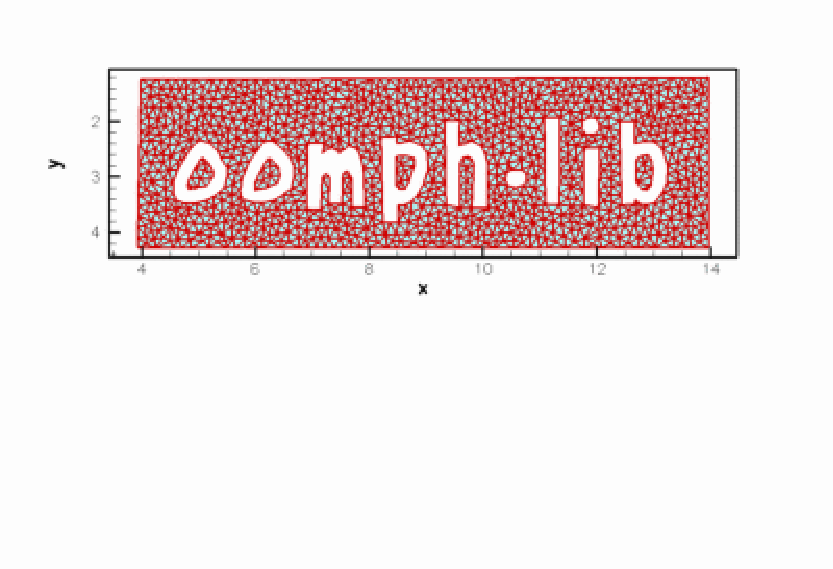
\includegraphics[width=0.75\textwidth]{oomph_mesh}}
\end{DoxyImageNoCaption}
   \\\cline{1-2}
\href{../../mesh_from_tetgen/html/index.html}{\tt {\bfseries  Tetgen\+Mesh$<$\+E\+L\+E\+M\+E\+N\+T$>$ }} ~\newline
~\newline

\begin{DoxyItemize}
\item This class creates {\ttfamily oomph-\/lib} meshes based on the output from \href{http://www.wias-berlin.de/~si }{\tt Hang Si\textquotesingle{}s} open-\/source mesh generator \href{http://wias-berlin.de/software/tetgen//}{\tt {\ttfamily Tetgen} }.
\item The mesh can be used with all {\ttfamily Finite\+Elements} that are derived from the geometric finite element {\ttfamily T\+Element$<$3,\+N\+N\+O\+D\+E\+\_\+1\+D$>$}.
\end{DoxyItemize}{\bfseries Example driver codes\+:} ~\newline

\begin{DoxyItemize}
\item The use of \href{http://wias-berlin.de/software/tetgen//}{\tt {\ttfamily Tetgen} } and the {\ttfamily Tetgen\+Mesh} class are explained in a \href{../../mesh_from_tetgen/html/index.html}{\tt separate tutorial.}
\end{DoxyItemize}& 
\begin{DoxyImageNoCaption}
  \mbox{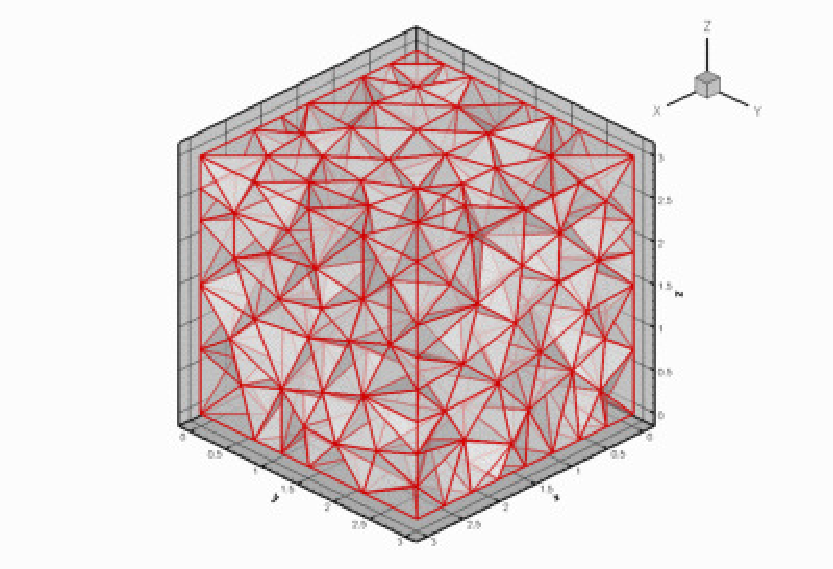
\includegraphics[width=0.75\textwidth]{tetgen_mesh}}
\end{DoxyImageNoCaption}
   \\\cline{1-2}
\href{../../mesh_from_vmtk/html/index.html}{\tt {\bfseries  Generating meshes from medical scans with V\+M\+TK }} ~\newline
~\newline

\begin{DoxyItemize}
\item We provide the option to generate tetgen-\/based meshes for physiological fluid-\/structure interaction problems, using the \href{http://www.vmtk.org}{\tt Vascular Modeling Toolkit (V\+M\+TK).}
\end{DoxyItemize}{\bfseries Example driver codes and tutorials\+:} ~\newline

\begin{DoxyItemize}
\item We provide a \href{../../mesh_from_vmtk/html/index.html}{\tt separate tutorial} that shows how to generate {\ttfamily oomph-\/lib} meshes from medical images.
\item The methodology is used in the following driver codes\+: ~\newline
~\newline

\begin{DoxyItemize}
\item \href{../../../solid/vmtk_solid/html/index.html}{\tt The inflation of a blood vessel.} ~\newline
~\newline

\item \href{../../../navier_stokes/vmtk_fluid/html/index.html}{\tt Finite Reynolds number flow through a (rigid) iliac bifurcation.} ~\newline
~\newline

\item \href{../../../interaction/vmtk_fsi/html/index.html}{\tt Finite Reynolds number flow through an elastic iliac bifurcation.} ~\newline
~\newline

\end{DoxyItemize}
\end{DoxyItemize}& 
\begin{DoxyImageNoCaption}
  \mbox{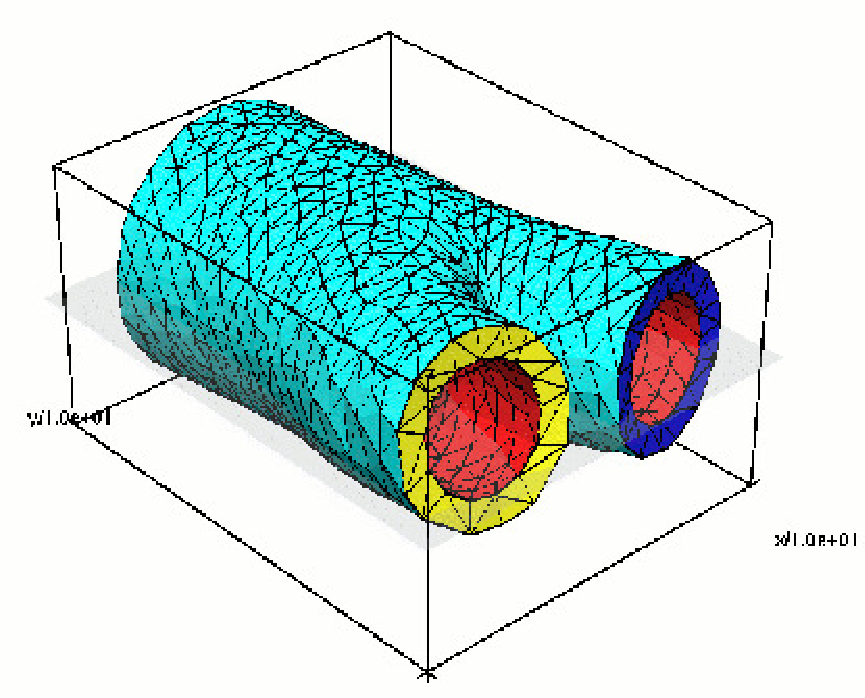
\includegraphics[width=0.75\textwidth]{iliac}}
\end{DoxyImageNoCaption}
   \\\cline{1-2}
\href{../../mesh_from_geompack/html/index.html}{\tt {\bfseries  Geompack\+Quad\+Mesh$<$\+E\+L\+E\+M\+E\+N\+T$>$ }} ~\newline
~\newline

\begin{DoxyItemize}
\item This class creates {\ttfamily oomph-\/lib} meshes based on the output from Barry Joe\textquotesingle{}s mesh generator \href{http://members.shaw.ca/bjoe/}{\tt {\ttfamily Geompack++}, } available as freeware at \href{http://members.shaw.ca/bjoe/}{\tt http\+://members.\+shaw.\+ca/bjoe/.}
\item The mesh can be used with all {\ttfamily Finite\+Elements} that are derived from the geometric finite element {\ttfamily Q\+Element$<$2,2$>$}.
\end{DoxyItemize}{\bfseries Example driver codes\+:} ~\newline

\begin{DoxyItemize}
\item The use of \href{http://members.shaw.ca/bjoe/}{\tt {\ttfamily Geompack++} } and the {\ttfamily Geompack\+Quad\+Mesh} class are explained in a \href{../../mesh_from_geompack/html/index.html}{\tt separate tutorial.}
\end{DoxyItemize}& 
\begin{DoxyImageNoCaption}
  \mbox{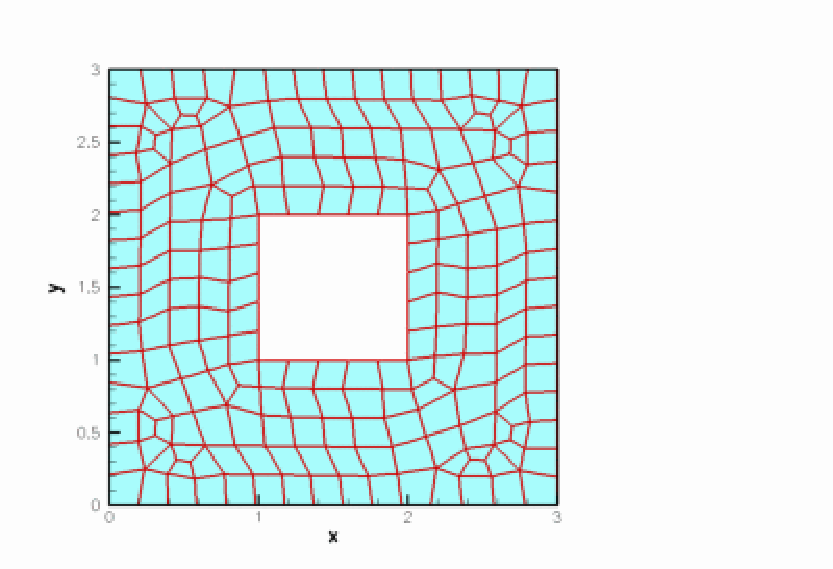
\includegraphics[width=0.75\textwidth]{geompack_mesh}}
\end{DoxyImageNoCaption}
   \\\cline{1-2}
\end{longtabu}
\end{center} 



 

 \hypertarget{index_pdf}{}\section{P\+D\+F file}\label{index_pdf}
A \href{../latex/refman.pdf}{\tt pdf version} of this document is available. \end{document}
